\chapter{Timing attacks}
	\index{Timing attacks}Come anticipato nel capitolo precedente, approfondiremo adesso la tipologia di attacchi basati sul tempo focalizzandoci maggiormente su quelli che hanno come obiettivo la cache del processore. 
	
	L'idea di base che sta sotto i timing attacks si basa sul fatto che l'esecuzione di un determinato programma, al variare delle operazioni che vengono eseguite e al variare degli input, impiega tempi diversi per portare a termine il proprio compito.
	
	\lstinputlisting[language={Java}, caption={Esempio di funzione vulnerabile ad un timing attack}, label={list:timingBase}, frame={none},basicstyle={\small\ttfamily}]{code/timingBase.txt}
		
	Ad esempio il \cref{list:timingBase} se fatto girare con la stringa ("passwordToBeStolen") impiegherà un tempo maggiore rispetto allo stesso programma fatto girare con la stringa ("foo"). Nel primo caso infatti verrà scansionata tutta la stringa mentre nel secondo caso si interromperà immediatamente. Questa informazione può essere utilizzata dall'attaccante che, procedendo per tentativi, può arrivare a ricavare la stringa esatta. Per portare questo concetto al livello che ci interessa vediamo prima delle nozioni fondamentali sulla cache del processore. 
	
	\section{La cache del processore}
		Solitamente, ogni programma, tende a riutilizzare, nel tempo, un dato contenuto allo stesso indirizzo di memoria (\emph{località temporale}\index{Località temporale}) e più dati localizzati in indirizzi vicini nella memoria (\emph{località spaziale}\index{Località spaziale}). Ad esempio, se nel programma è presente un loop, lo stesso codice sarà eseguito più e più volte nel tempo verosimilmente con gli stessi dati.
		
		Dato che la differenza di velocità tra le memorie e la capacità di calcolo dei processori aumenta sempre di più \cite{hennessy2011computer}, la banda del bus di comunicazione e la velocità di accesso alla memoria principale sono diventati un fattore limitante sul throughput generale del processore. Per sfruttare al meglio la località temporale e superare questo collo di bottiglia vengono utilizzate le caches\index{Cache}. 
		
		La cache è infatti un piccolo banco di memoria molto veloce sito all'interno di ogni core che il processore utilizza per immagazzinare i valori delle celle di memoria accedute più recentemente. 
		
		\subsection{Struttura della cache}
			I processori moderni hanno generalmente due livelli di cache per ogni core chiamati rispettivamente L1 e L2 ed un terzo livello chiamato \ac{LLC} o L3 condiviso tra i tutti i core (nella \cref{tab:processori} sono riportate le dimensioni delle varie memorie di alcuni processori). 
			
			\begin{table}[]
				\footnotesize
				\centering
				\begin{tabular}{|c|c|c|c|c|c|c|} \hline
					Casa		& Nome			& Core	& L1			& L2			& L3		& Prezzo (\$)	\\ \hline \hline
					Intel		& i3-530		& 2		& 2 x 64 KB		& 2 x 512KB		& 1 x 4 MB	& 113			\\ \hline
								& i5-6685R		& 4		& 4 x 64 KB		& 4 x 256KB		& 1 x 6 MB	& 288			\\ \hline
								& i7-6950X		& 10	& 10 x 64 KB	& 10 x 256KB	& 1 x 25 MB	& 1723			\\ \hline
								& i9-8950HK		& 6		& 6 x 64 KB		& 6 x 256KB		& 1 x 12 MB	& 583			\\ \hline
					AMD			& A4 Pro-3350B	& 4		& 4 x 64 KB		& 1 x 2MB		& -			& -				\\ \hline
								& Athlon 5370	& 4		& 4 x 64 KB		& 1 x 2MB		& -			& 55			\\ \hline
								& Epyc 7251		& 8		& 8 x 96 KB		& 8 x 512KB		& 32 MB		& 475			\\ \hline
				\end{tabular}
				\caption{Caratteristiche di alcuni processori}
				\label{tab:processori}
			\end{table}
			
			Considerando che l'accesso alla memoria principale in media impiega dai $50$ ai $150$ \emph{ns} mentre l'accesso alla cache L1 utilizza un tempo nell'ordine degli $0.3$ \emph{ns} si può capire l'enorme differenza di prestazioni che possono essere raggiunte utilizzando questo tipo di memoria.
		
			Nella \cref{fig:cachei5} si può vedere l'architettura del processore quadcore Intel Core i5-3470. La gerarchia delle cache è organizzata in una memoria L1 di 64KB (divisa in 32KB per le istruzioni e 32KB per i dati), una memoria L2 da 256KB ed una memoria L3 da 6MB.
			
			\begin{figure}
				\begin{center}
					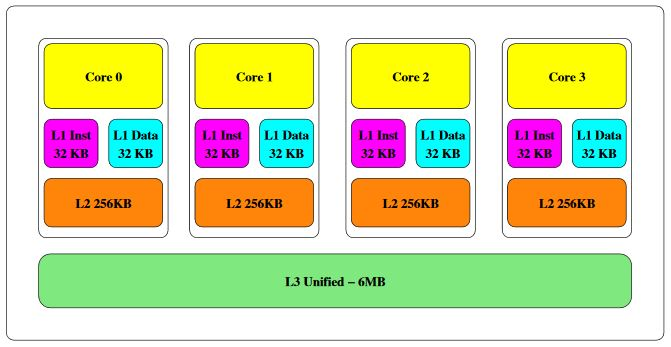
\includegraphics[scale=0.6]{cachei5}
					\caption{Architettura del processore Intel Core i5-3470}
					\label{fig:cachei5}
				\end{center}
			\end{figure}
			
			Andiamo ad analizzare più nel dettaglio le caratteristiche di una singola cache\cite{ge2016survey,yarom2014flush+}.
			
			\subsubsection{Cache lines}
				\index{Cache lines}Per sfruttare anche la località spaziale le caches sono divise in lines. Una cache line contiene un blocco di byte adiacenti (generalmente di dimensione congrua ad una potenza di due) caricati dalla memoria. Se uno qualunque dei byte deve essere rimosso (si parla di \emph{evicting}\index{Evict}) per far spazio ad un altro dato, viene rimossa l'intera line.
				
			\subsubsection{Associatività}
				Teoricamente una qualunque posizione di memoria può essere mappata in una qualunque cache line ed una cache ad \emph{n} lines potrebbe contenere \emph{n} linee qualunque dalla memoria. Questo tipo di cache viene chiamato \emph{fully-associative cache}\index{Fully-associative cache} ed è la migliore in teoria perché può sempre essere usata al massimo delle sue capacità e i cache miss si hanno solamente quando non c'è più spazio libero nella cache. In pratica però questo si traduce in un controllo in parallelo di tutte le linee che aumenta la complessità architetturale e il consumo di energia.
				
				L'estremo opposto è chiamato \emph{direct-mapped cache}\index{Direct-mapped cache}. In questo sistema ogni locazione di memoria può stare in una sola cache line, ben determinata da una funzione di indicizzazione. Due locazioni di memoria che mappano sulla stessa cache line non possono essere immagazzinate contemporaneamente e il loading di una comporta inevitabilmente l'evicting dell'altra. Questo potrebbe portare ad avere dei miss anche con la cache semivuota.
				
				\begin{figure}
					\begin{center}
						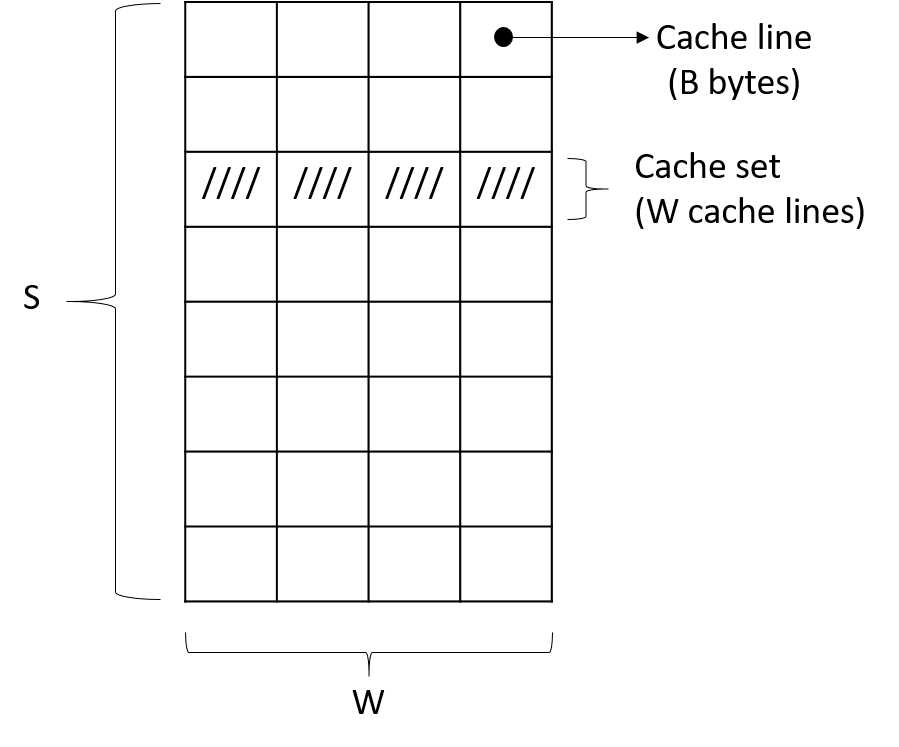
\includegraphics[scale=.5]{cache}
						\caption{Un esempio di 8-way associative cache con otto set formati ognuno da 4 line.}
						\label{fig:cache}
					\end{center}
				\end{figure}
				
				Concretamente viene utilizzata una via di mezzo tra queste due soluzioni chiamata \emph{set-associative cache}\index{Set-associative cache}. La cache viene divisa in \emph{sets} (generalmente di dimensione compresa tra due e ventiquattro lines) in cui ogni indirizzo viene controllato in parallelo come in una fully-associative cache. In quale set viene mappato un blocco di memoria viene calcolato come per una direct-mapped cache da una funzione del suo indirizzo. Una cache con \emph{S} line sets viene chiamata \emph{S-way associative}(\cref{fig:cache}). 
				
				In \cref{fig:cachefill} possiamo vedere un esempio di direct-mapped e 2-way associative cache. 
				
				Nella prima, la funzione di indicizzazione potrebbe essere: $$\text{cache memory index} = \text{main memory index}\ \% \ 4$$ Supponiamo adesso che in cache sia presente il dato \emph{x} contenuto all'indirizzo $0$ della memoria principale. La richiesta del dato \emph{y} contenuto all'indirizzo 4 provocherà l'evict di \emph{x}.
				
				Nella seconda, la funzione di indicizzazione potrebbe essere: $$\text{cache memory index} = \text{main memory index}\ \% \ 2$$ In questo caso però, dal momento che per ogni set è possibile salvare due line contemporaneamente, la richiesta del dato \emph{y} non provocherebbe l'evict del dato \emph{x} già presente in cache ma sarebbero entrambi presenti in cache, nel set $0$, l'uno con indice $0$ e l'altro con indice 1.
				
				Si può notare che le direct-mapped e le fully-associative cache non sono altro che casi particolari di set-associative cache, rispettivamente 1-way associative ed N-way associative (dove N è il numero totale di linee della cache).
				
				\begin{figure}
					\begin{center}
						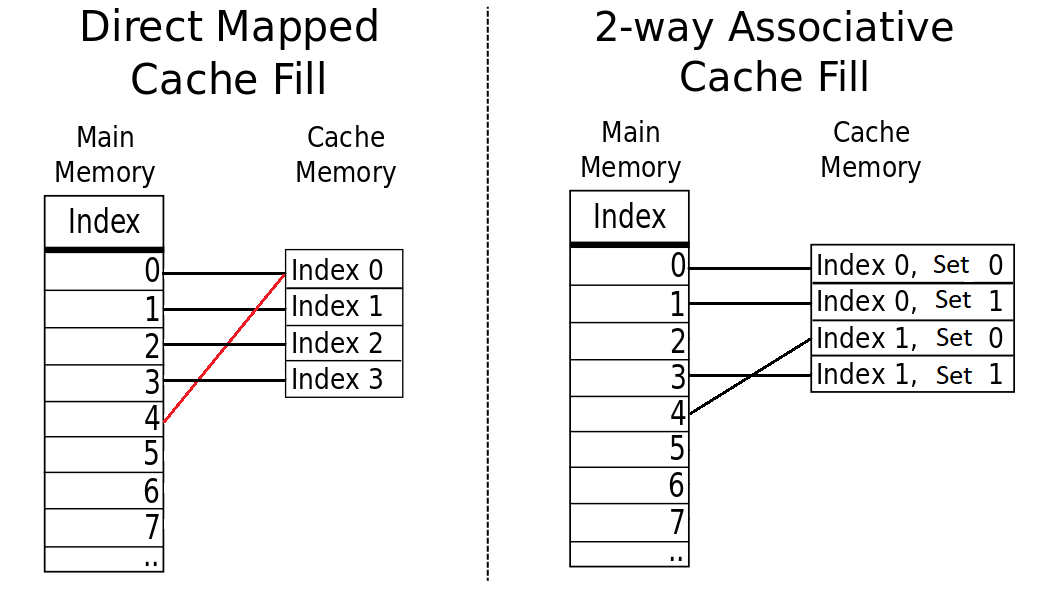
\includegraphics[scale=.35]{cachefill}
						\caption{Schemi di associatività della cache.}
						\label{fig:cachefill}
					\end{center}
				\end{figure}
				
			\subsubsection{Inclusività}
				Una caratteristica che verrà sfruttata per montare l'attacco è l'\emph{inclusività}\index{Inclusività}. 
				
				Ogni livello superiore di cache contiene un sottoinsieme dei dati contenuti dal livello direttamente inferiore. Per mantenere questa caratteristica, quando viene eseguito un evicting di un dato da un livello inferiore, questo viene rimosso anche da tutti i livelli superiori.
				
				Se ad esempio effettuiamo un evicting di una line contenuta nella cache L3, lo stesso dato, se presente, verrà rimosso anche dalla L1 e dalla L2.
				
	\section{Cache attacks}
		Per capire come funzionano la maggior parte degli attacchi alle cache prendiamo in considerazione un array di dati. Quando un elemento di questo array viene acceduto possono verificarsi una di queste due condizioni:
		
		\begin{enumerate}
			\item Il dato è presente in cache, si verifica una hit e viene recuperato molto velocemente.
			\item Il dato non è presente in cache, si verifica una miss e bisogna aspettare che venga recuperato dalla memoria principale.
		\end{enumerate}
		
		La differenza tra le due esecuzioni è notevole (diversi ordini di grandezza) ed è questa l'informazione utilizzata nell'attacco.
		
		\subsection{Tassonomia}
			Una prima classificazione dei cache attacks si basa sullo stato della cache al momento dell'attacco\cite{canteaut2006understanding}.
			
			\begin{itemize}
				\item \emph{Empty initial state}\index{Empty initial state} (reset attacks): questi attacchi si basano sull'assunzione che nessun dato che dovrà essere utilizzato dalla vittima è presente in cache.
				\item \emph{Forged initial state}\index{Forged initial state} (initialization attacks): in questo caso l'attaccante deve essere in grado di portare la cache in uno stato noto prima di poter effettuare l'attacco.
				\item \emph{Loaded initial state}\index{Loaded initial state} (micro-architecture attacks): la cache contiene tutti i dati necessari alla vittima per eseguire il programma.
			\end{itemize}
		
			Nello stesso lavoro si fornisce una classificazione anche in base al tipo di cache miss. 
			
			\begin{itemize}
				\item \emph{Cold start misses}\index{Cold start misses}: questo tipo di miss si ottiene quando il dato viene acceduto per la prima volta e quindi non è ancora mai stato caricato in cache.
				\item \emph{Capacity misses}\index{Capacity misses}: questo tipo di miss si ottiene quando si cerca di accedere a porzioni di memoria più grandi della dimensione della cache che quindi non possono essere presenti contemporaneamente.
				\item \emph{Conflict misses}\index{Conflict misses}: questo tipo di miss si ottiene quando un accesso precedente alla nostra richiesta ha provocato la eviction del dato di interesse (che era presente in cache).
			\end{itemize}
			
			In \cite{lipp2016armageddon,ge2016survey} si classificano gli attacchi in base all'approccio utilizzato:
			
			\begin{figure}
				\begin{center}
					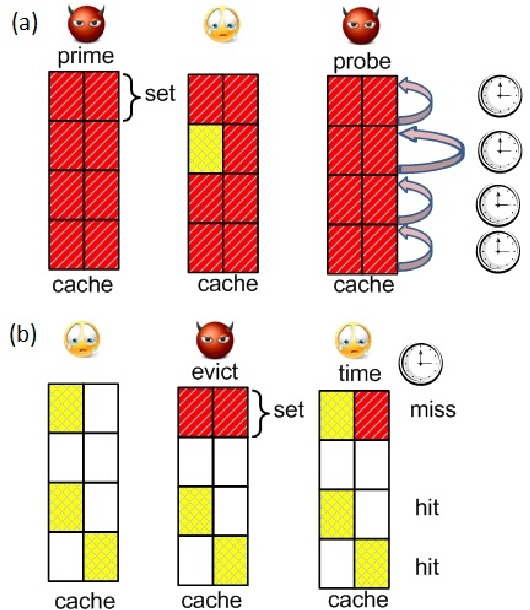
\includegraphics[scale=0.4]{cacheattacks}
					\caption{Schema di attacco Prime+Probe (a) e Evict+Time(b)}
					\label{fig:cacheattacks}
				\end{center}
			\end{figure}
			
			\begin{itemize}
				\item \emph{Prime+Probe}\cite{osvik2006cache}\index{Prime+Probe}: Questo è un attacco di tipo forged initial state. L'attaccante precarica uno o più set della cache con dati propri. Dopo l'esecuzione della funzione vittima prova a riaccedere ai propri dati. Se la funzione vittima non ha utilizzato lines mappate nei cache set occupati dall'attaccante, egli otterrà solo cache hit. Al contrario, se c'è stato l'evict di qualche line allora capirà quale ha utilizzato la vittima. Lo schema di questo attacco e del seguente è visibile in \cref{fig:cacheattacks}.
				\item \emph{Evict+Time}\cite{osvik2006cache}\index{Evict+Time}: Questo attacco è di tipo loaded initial state e suppone che tutti i dati che servono alla vittima siano già in cache. Questa condizione può essere ottenuta facendo eseguire una prima volta la funzione vittima. Con questa base, l'attaccante fa eseguire la funzione alla vittima calcolandone il tempo di esecuzione. Successivamente esegue una evict di un cache set caricando dati propri e fa eseguire nuovamente la funzione vittima. Se il tempo di questa ultima esecuzione è maggiore del precedente vuol dire che la funzione ha cercato di utilizzare un dato che è stato rimosso dalla cache ed ha dovuto aspettare di recuperarlo dalla memoria principale.
				\item \emph{Flush+Reload}\cite{yarom2014flush+}\index{Flush+Reload}: Questo attacco è una variante di Prime+Probe. L'attacco si divide in tre fasi. Nella prima fase l'attaccante esegue l'evict della linea a cui è interessato utilizzando l'istruzione \emph{clflush}\cite{intel64and}\index{Clflush} che invalida il dato su tutti i livelli della cache. Nella seconda fase aspetta che la vittima esegua la propria funzione. Nella terza fase l'attaccante ricarica la linea che aveva rimosso. Se la risposta è veloce vuol dire che la vittima l'ha portata in cache durante l'esecuzione della sua funzione.
				\item \emph{Evict+Reload}\cite{gruss2015cache}\index{Evict+Reload}: Una variante del Flush+Reload che utilizza la eviction al posto dell'istruzione di flush. Questa variante è poco utile se il processore sotto attacco è della famiglia x86 in quanto l'istruzione \emph{clflush} non richiede alcun privilegio mentre assume un certo rilievo se l'obiettivo è quello di attaccare un processore che non fornisce, nel suo set di istruzioni, una istruzione non privilegiata in grado di rimuovere dati dalla cache (come ad esempio quelli della famiglia ARM).
				\item \emph{Flush+Flush}\cite{gruss2016flush+}\index{Flush+Flush}: Diversamente da tutti i precedenti approcci, in questo caso non si esegue nessun accesso alla memoria ma l'attaccante si basa solamente sul tempo impiegato dall'istruzione \emph{clflush}. In \cite{lipp2016armageddon} si fa vedere come l'esecuzione di questa funzione abbia tempi differenti se chiamata su un indirizzo presente in cache o meno.  
			\end{itemize}
		
		\section{L'attacco ad AES}
			Un ottimo esempio di come sono stati messi in pratica buona parte dei concetti visti fino ad ora è l'attacco ad \ac{AES} portato da \emph{Osvik, Shamir \text{e} Tromer} in \cite{osvik2006cache}.
			
			\subsection{AES}
				\ac{AES}\index{AES} è un algoritmo di cifratura a blocchi, a chiave simmetrica, scelto come standard dagli Stati Uniti d'America dalla \ac{FIPS} nel documento PUB 197\cite{pub2001197}. Viene considerato a tutti gli effetti il successore di \ac{DES}, in via di abbandono a causa della sua ormai provata insicurezza\cite{kumar2006breaking,gilmore1998cracking}. La rimanente spiegazione dell'algoritmo è presa da \cite{stallings2012computer}.
				
				\ac{AES} utilizza blocchi di 128 bit e una chiave che può essere lunga 128, 192 o 256 bit (128 è la lunghezza più comunemente implementata).
			
				L'input dell'algoritmo è un singolo blocco di 128 bit che nello standard viene trattato come una matrice quadrata di byte (come la chiave a 128 bit). Questo blocco viene copiato in un array chiamato \emph{stato} che verrà modificato ad ogni round di encryption/decryption. Alla fine dell'ultimo round, lo stato finale sarà copiato in una matrice che rappresenterà il risultato della computazione. La chiave viene espansa in un array di word (della lunghezza di quattro byte) ricavando 44 word dai 128 bit di partenza. Ad ogni round verranno prese di volta in volta quattro word (128 bit) e verranno utilizzate come chiave per quel round.
				
				Senza scendere troppo nell'implementazione è importante capire le quattro operazioni effettuate ad ogni round(\cref{fig:operations}):
				
				\begin{itemize}
					\item \emph{Substitute byte}: tramite una tabella (\emph{S-Box}) vengono sostituiti, byte per byte, tutti i byte del blocco.
					\item \emph{Shift row}: viene effettuata una permutazione delle righe della matrice
					\item \emph{Mix columns}: vengono modificate le colonne moltiplicandole per un polinomio fisso $c(x)$.
					\item \emph{Add round key}: viene effettuato uno XOR tra il blocco corrente e la chiave di round.
				\end{itemize}
			
				\begin{figure}
					\begin{center}
						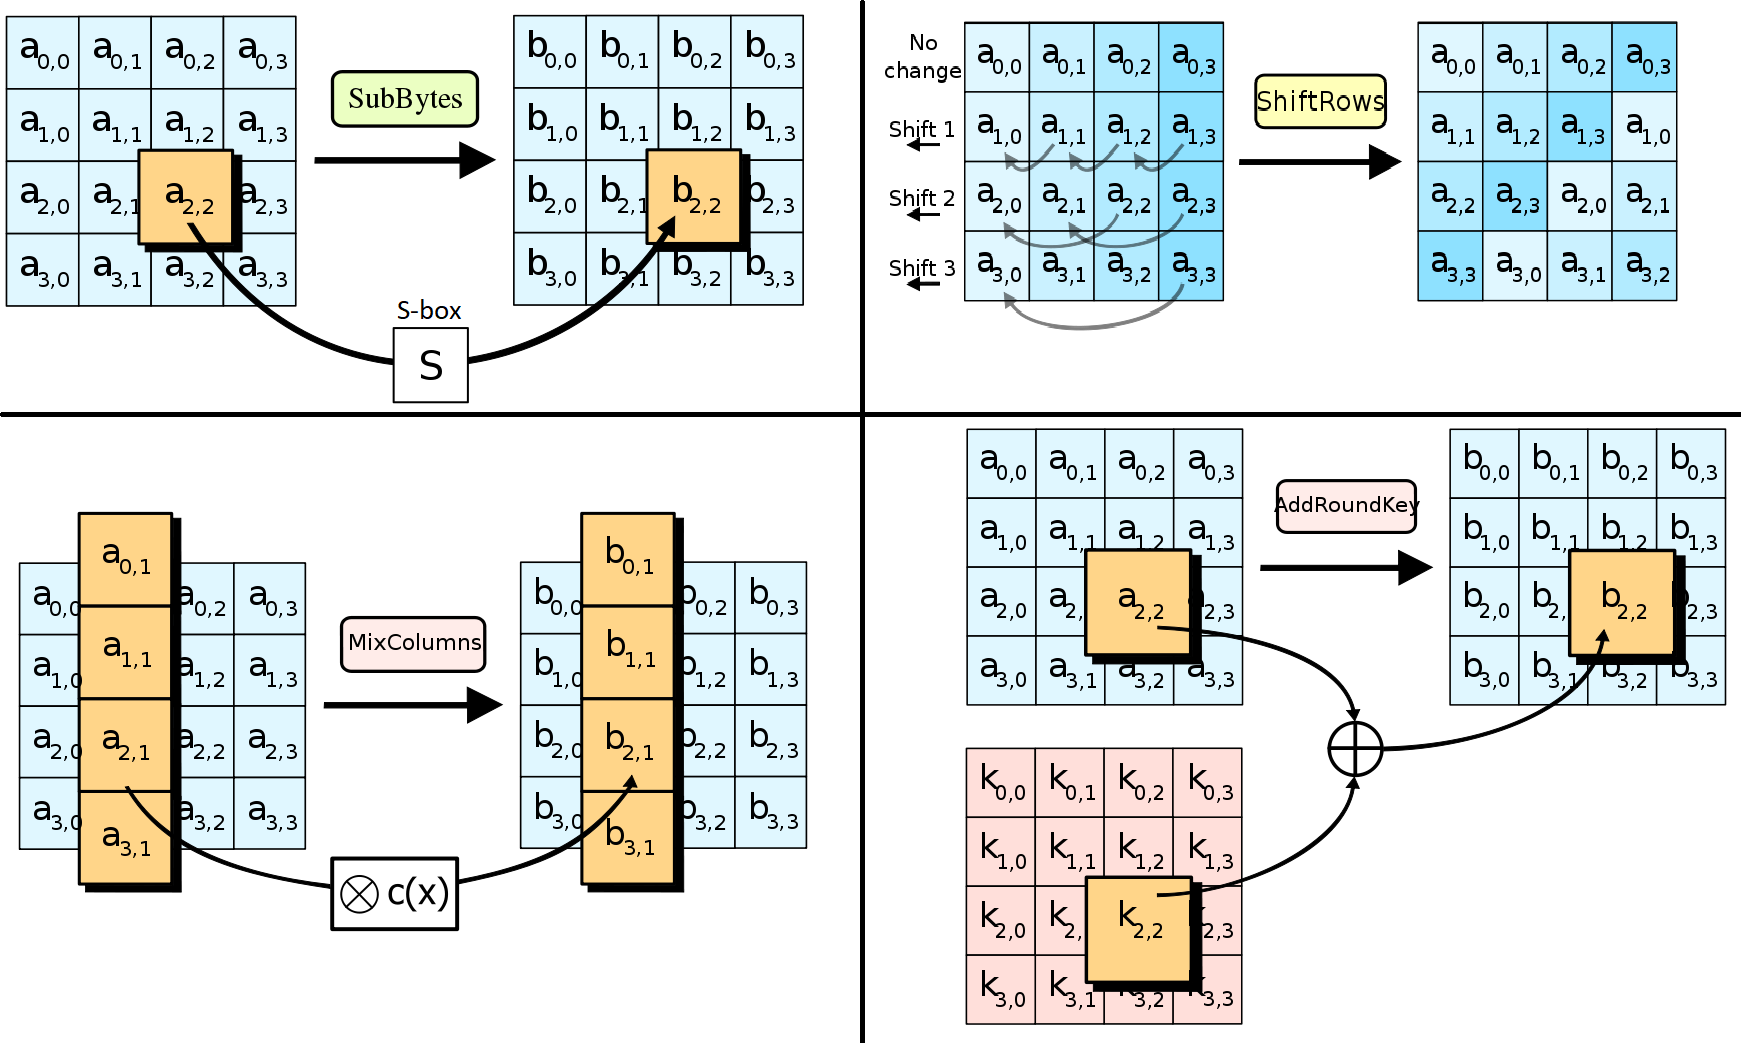
\includegraphics[width=\textwidth]{aesOperations}
						\caption{Schema delle operazioni effettuate da AES}
						\label{fig:operations}
					\end{center}
				\end{figure}
			
				Come si vede in \cref{fig:aes} l'algoritmo inizia con un \emph{add round key} seguito da nove round in cui vengono effettuate tutte e quattro le operazioni. L'ultimo round (il decimo) è composto da solo tre di queste in quanto non viene effettuata la \emph{mix columns}.
				
				\begin{figure}
					\begin{center}
						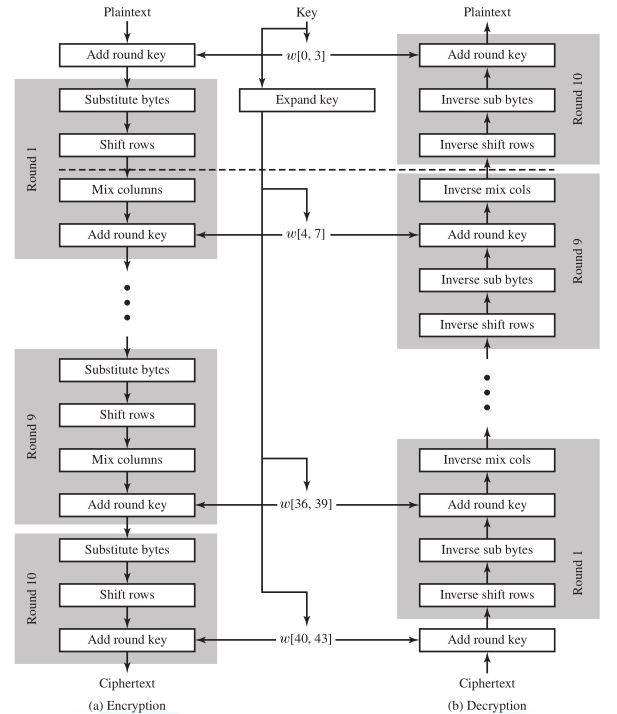
\includegraphics[width=.9\textwidth]{AES}
						\caption{Schema di funzionamento di AES}
						\label{fig:aes}
					\end{center}
				\end{figure}
				
			\subsection{Implementazione e uso della memoria}
				Quello descritto fino a qui è il funzionamento teorico di \ac{AES}; teoricamente, tutto l'algoritmo è eseguibile tramite semplici operazioni algebriche ma in realtà, per migliorare le performance, vengono create (dal programmatore o durante l'inizializzazione del sistema) otto tabelle di lookup che chiameremo $\mathcal{T}_0, \mathcal{T}_1, \mathcal{T}_2, \mathcal{T}_3$ e $\mathcal{T}_{0}^{(10)}, \mathcal{T}_{1}^{(10)}, \mathcal{T}_{2}^{(10)}, \mathcal{T}_{3}^{(10)}$. Ognuna di queste tabelle contiene 256 word da quattro byte. La chiave (sedici byte) $\mathbf{k} = (k_1,\dots ,k_{16})$ viene estesa per formare dieci chiavi (una per ogni round) $\mathbf{K}^{(r)}$ per $r = 1,\dots ,10$ che vengono suddivise in quattro word di quattro byte ciascuna $\mathbf{K}^{(r)}=\left( K_{0}^{(r)},K_{1}^{(r)},K_{2}^{(r)},K_{3}^{(r)}\right) $. Dato un plaintext di sedici byte $\mathbf{p}=(p_0, \dots , p_{15})$ la funzione di encryption calcola uno stato intermedio $\mathbf{x}^{(r)}=(x_{0}^{(r)}, \dots , x_{15}^{(r)})$ ad ogni round r. Lo stato iniziale $\mathbf{x}^{(0)}$ viene calcolato come $x_{i}^{(0)} = p_i \oplus k_i \text{ con }(i = 0,\dots ,15)$. I nove round seguenti vengono calcolati aggiornando lo stato intermedio secondo le seguenti equazioni (per $r = 0,\dots,8$):
				{
					\scriptsize
					\begin{center}
						\begin{tabular}{ccc}
							$\left(x_{0}^{(r+1)},x_{1}^{(r+1)},x_{2}^{(r+1)},x_{3}^{(r+1)}\right)$ & $\leftarrow$ & $\mathcal{T}_{0}\left[x_{0}^{(r)}\right] \oplus \mathcal{T}_{1}\left[x_{5}^{(r)}\right] \oplus \mathcal{T}_{2}\left[x_{10}^{(r)}\right] \oplus \mathcal{T}_{3}\left[x_{15}^{(r)}\right]\oplus K_{0}^{(r+1)}$\\
							$\left(x_{4}^{(r+1)},x_{5}^{(r+1)},x_{6}^{(r+1)},x_{7}^{(r+1)}\right)$ & $\leftarrow$ & $\mathcal{T}_{0}\left[x_{4}^{(r)}\right] \oplus \mathcal{T}_{1}\left[x_{9}^{(r)}\right] \oplus \mathcal{T}_{2}\left[x_{14}^{(r)}\right] \oplus \mathcal{T}_{3}\left[x_{3}^{(r)}\right]\oplus K_{1}^{(r+1)}$\\
							$\left(x_{8}^{(r+1)},x_{9}^{(r+1)},x_{10}^{(r+1)},x_{11}^{(r+1)}\right)$ & $\leftarrow$ & $\mathcal{T}_{0}\left[x_{8}^{(r)}\right] \oplus \mathcal{T}_{1}\left[x_{13}^{(r)}\right] \oplus \mathcal{T}_{2}\left[x_{2}^{(r)}\right] \oplus \mathcal{T}_{3}\left[x_{7}^{(r)}\right]\oplus K_{2}^{(r+1)}$\\
							$\left(x_{12}^{(r+1)},x_{13}^{(r+1)},x_{14}^{(r+1)},x_{15}^{(r+1)}\right)$ & $\leftarrow$ & $\mathcal{T}_{0}\left[x_{12}^{(r)}\right] \oplus \mathcal{T}_{1}\left[x_{1}^{(r)}\right] \oplus \mathcal{T}_{2}\left[x_{6}^{(r)}\right] \oplus \mathcal{T}_{3}\left[x_{11}^{(r)}\right]\oplus K_{3}^{(r+1)}$
						\end{tabular}
					\end{center}
				}
			
				L'ultimo round viene calcolato con $r = 9$ ma, al posto di usare $\mathcal{T}_0, \mathcal{T}_1, \mathcal{T}_2, \mathcal{T}_3$ verranno usate $\mathcal{T}_{0}^{(10)}, \mathcal{T}_{1}^{(10)}, \mathcal{T}_{2}^{(10)}, \mathcal{T}_{3}^{(10)}$. Il risultante $\mathbf{x}^{10}$ sarà il ciphertext.
				
				Paragonando questa implementazione con la formulazione algebrica teorica di \ac{AES} si può vedere che le otto tabelle di lookup vengono usate per effettuare le quattro operazioni di ogni round in maniera immediata. L'ultimo round ha bisogno di quattro tabelle diverse perché non viene eseguita l'operazione \emph{mix columns}.
				
				L'attacco (i cui dettagli possono essere trovati nell'articolo) si basa proprio sul cercare di capire i valori $x_{i}^{(r)}$ usati come indici nelle varie tabelle che di volta in volta verranno caricate in cache. Tali valori vengono recuperati tramite attacchi evict+time o prime+probe.
		
		\section{Contromisure possibili}
			Le difese da questo tipo di attacchi sono sia software che hardware e si dividono in cinque grandi famiglie\cite{ge2016survey}
			
			\begin{description}
				\item[Tecniche a tempo costante:] L'idea di base è quella di rendere il comportamento del codice che esegue operazioni critiche indipendente dai dati. Per esempio cercare di rendere una funzione crittografica indipendente sia dalla chiave che dall'input. Questo può essere ottenuto facendo eseguire istruzioni inutili per uniformare il tempo di esecuzione o accedendo a dati casuali dalla memoria per confondere l'attaccante sull'utilizzo della cache. 
				
				Queste soluzioni ovviamente portano ad una drastica perdita di prestazioni. Il tempo di esecuzione dovrà infatti tendere al tempo di esecuzione massimo ogni volta che sarà necessario richiamare la funzione.
				
				L'altro grande problema di questo tipo di soluzioni è quello della differenza di risultati su hardware differenti. Ad esempio \emph{Cock et al.}\cite{cock2014last} hanno dimostrato che la correzione a tempo costante adottata per mitigare l'attacco \emph{Lucky 13}\cite{al2013lucky} in OpenSSL $1.0.1$e non risolve il problema se fatto girare su un processore ARM AM3358. 
				\item[Inserimento di rumore:] Questa famiglia di contromisure tende a rendere inutilizzabili le misurazioni ottenute dall'attaccante inserendo in ogni evento osservabile da qualsiasi processo una quantità di rumore tale da renderne impossibile una qualunque analisi\cite{hu1992reducing}. Questa soluzione, in teoria, riesce a risolvere completamente il problema ma è stato dimostrato\cite{cock2014last} che in pratica non è applicabile. La quantità di rumore da produrre e da aggiungere alla computazione è talmente elevata che il sistema impiegherebbe la maggior parte delle sue risorse in questa operazione piuttosto che nella effettiva computazione del programma.
				\item[Imporre determinismo:] In questo caso si cerca di eliminare qualsiasi tipo di misura sul tempo eliminando completamente le variazioni di tempo visibile. Ad esempio in \cite{aviram2012efficient} si propone di eliminare completamente l'accesso al tempo reale fornendo all'esterno solamente un clock virtuale il cui avanzamento è completamente deterministico e indipendente dalle azioni di componenti vulnerabili. Per ottenere questo risultato si cerca di sincronizzare tutti i clock con l'esecuzione di un singolo processo, indipendente da input o azioni esterne, che esegue in tempo costante.
				\item[Suddividere il tempo:] Una delle soluzioni maggiormente utilizzate è quella in cui si cerca di suddividere il tempo in sezioni nelle quali si fornisce un accesso esclusivo all'hardware condiviso. Ci sono diverse tecniche per ottenere questo risultato uno dei quali è lo svuotamento completo della cache ad ogni context switch (\emph{cache flushing}\index{Cache flushing}\cite{zhang2013duppel}). Questo ovviamente porta ad una perdita in prestazioni molto grande e si è passati al \emph{lattice scheduling}\index{Lattice scheduling}\cite{denning1976lattice} che esegue il flushing della cache non ad ogni context switch ma solo nel passaggio da processi sensibili a processi inaffidabili. Un'altra soluzione\cite{varadarajan2014scheduler} mira a sfruttare la necessità di analizzare molto spesso lo stato della cache della vittima. Tale necessità è richiesta dagli attacchi di tipo Prime+Probe ad esempio e non viene soddisfatta imponendo un tempo minimo di esecuzione per le componenti vulnerabili entro il quale non possono essere prelazionate.
				\item[Suddividere le risorse hardware:] Attacchi eseguiti da processi concorrenti possono essere evitati solamente suddividendo adeguatamente le risorse hardware tra i vari processi. Per quanto riguarda la cache sono state avanzate varie proposte. Percival\cite{percival2005cache} suggerisce di suddividere la cache L1 tra i vari processi in modo tale da non permettere ad un processo di accedere o rimuovere lines utilizzate da un altro. Wang e Lee\cite{wang2007new} propongono invece la \emph{partition-locked cache}, un meccanismo hardware che permette di assegnare dei lock ad alcune lines contenenti dati particolarmente sensibili in maniera tale da non poter essere rimosse (ad esempio le tabelle di lookup di \ac{AES}).				 
			\end{description}